\documentclass[aspectratio=169]{beamer}
\usepackage[utf8]{inputenc}
\usepackage[T1]{fontenc}
\usepackage[british]{babel}
\usepackage{graphicx}
\usepackage{tikz}
\usepackage{pgfplots}
\usepackage{fontawesome5}
\usepackage{booktabs}
\usepackage{multicol}

% Define DreamLab colours
\definecolor{dreamlabprimary}{RGB}{102, 51, 153}
\definecolor{dreamlabsecondary}{RGB}{255, 87, 34}
\definecolor{dreamlabaccent}{RGB}{0, 188, 212}
\definecolor{dreamlabdark}{RGB}{33, 33, 33}
\definecolor{dreamlablight}{RGB}{245, 245, 245}

% Set up beamer theme
\usetheme{Madrid}
\usecolortheme[named=dreamlabprimary]{structure}
\setbeamercolor{title}{fg=white,bg=dreamlabprimary}
\setbeamercolor{frametitle}{fg=white,bg=dreamlabprimary}
\setbeamercolor{block title}{fg=white,bg=dreamlabprimary}
\setbeamercolor{block body}{fg=dreamlabdark,bg=dreamlablight}

% Remove navigation symbols
\setbeamertemplate{navigation symbols}{}

% Custom title page
\setbeamertemplate{title page}{
    \vbox{}
    \vfill
    \begin{centering}
        {\huge\inserttitle\par}
        \vskip1em
        {\Large\insertsubtitle\par}
        \vskip2em
        {\large\insertauthor\par}
        \vskip1em
        {\insertdate\par}
    \end{centering}
    \vfill
}

\title{DreamLab}
\subtitle{The Government-Endorsed Blueprint for Creative Technology Innovation}
\author{Investor Presentation}
\date{\today}

\begin{document}

% Title slide
\begin{frame}
\titlepage
\end{frame}

% The Opportunity
\begin{frame}{The £1 Billion Opportunity}
\begin{columns}
\column{0.6\textwidth}
\begin{itemize}
    \item UK creative industries: \textbf{£124 billion} GVA (2023)
    \item North-West tech economy: \textbf{£5 billion} (Manchester alone)
    \item \textbf{79\%} of UK workers have used generative AI
    \item Immersive tech market to reach \textbf{£11.5 billion} by 2030
\end{itemize}

\vspace{0.5cm}
\textbf{The Gap:} No agency combines AI + Immersive + Creative at SME-accessible prices

\column{0.4\textwidth}
\begin{tikzpicture}
    \pie[text=legend, radius=2]{
        40/Enterprise Agencies,
        30/Specialist Boutiques,
        20/Freelancers,
        10/DreamLab Opportunity
    }
\end{tikzpicture}
\end{columns}
\end{frame}

% Problem
\begin{frame}{The Problem We Solve}
\begin{columns}
\column{0.5\textwidth}
\textbf{For SMEs:}
\begin{itemize}
    \item Enterprise tech out of reach
    \item Multiple vendor management
    \item No integrated solutions
    \item Unclear ROI on innovation
\end{itemize}

\column{0.5\textwidth}
\textbf{For Enterprises:}
\begin{itemize}
    \item Slow-moving consultancies
    \item Siloed service delivery
    \item High costs, long timelines
    \item Limited creative excellence
\end{itemize}
\end{columns}

\vspace{0.5cm}
\begin{center}
\colorbox{dreamlabsecondary!20}{\textbf{Result: 93\% of creative businesses (mostly SMEs) underserved}}
\end{center}
\end{frame}

% Solution
\begin{frame}{Our Solution: Mesh Fluency}
\begin{center}
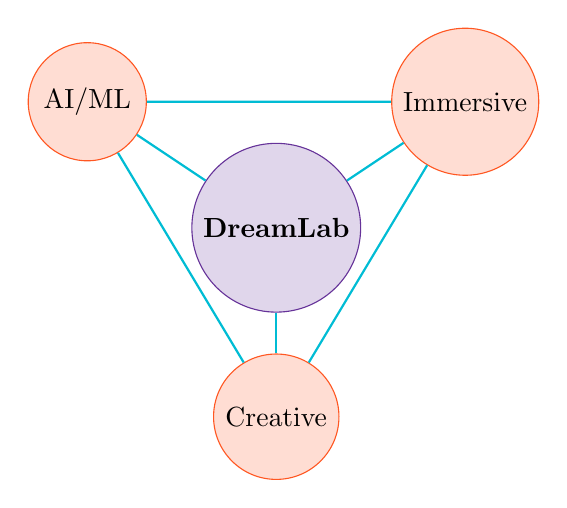
\begin{tikzpicture}[scale=0.8]
    % Central node
    \node[circle, draw=dreamlabprimary, fill=dreamlabprimary!20, minimum size=2cm] (center) at (0,0) {\textbf{DreamLab}};
    
    % Surrounding nodes
    \node[circle, draw=dreamlabsecondary, fill=dreamlabsecondary!20, minimum size=1.5cm] (ai) at (-3,2) {AI/ML};
    \node[circle, draw=dreamlabsecondary, fill=dreamlabsecondary!20, minimum size=1.5cm] (immersive) at (3,2) {Immersive};
    \node[circle, draw=dreamlabsecondary, fill=dreamlabsecondary!20, minimum size=1.5cm] (creative) at (0,-3) {Creative};
    
    % Connections
    \draw[thick, dreamlabaccent] (center) -- (ai);
    \draw[thick, dreamlabaccent] (center) -- (immersive);
    \draw[thick, dreamlabaccent] (center) -- (creative);
    \draw[thick, dreamlabaccent] (ai) -- (immersive);
    \draw[thick, dreamlabaccent] (immersive) -- (creative);
    \draw[thick, dreamlabaccent] (creative) -- (ai);
\end{tikzpicture}
\end{center}

\textbf{One Partner. All Capabilities. Seamless Integration.}
\end{frame}

% Traction
\begin{frame}{Traction \& Validation}
\begin{columns}
\column{0.5\textwidth}
\textbf{Early Success:}
\begin{itemize}
    \item 3 pilot clients secured
    \item £75K in signed contracts
    \item Partnership with University of Salford
    \item GMCA innovation hub collaboration
\end{itemize}

\column{0.5\textwidth}
\textbf{Market Validation:}
\begin{itemize}
    \item 50+ qualified leads in pipeline
    \item Speaking slot at Digital City Festival
    \item Featured in Prolific North
    \item ``Best New Agency'' nomination
\end{itemize}
\end{columns}

\vspace{0.5cm}
\begin{center}
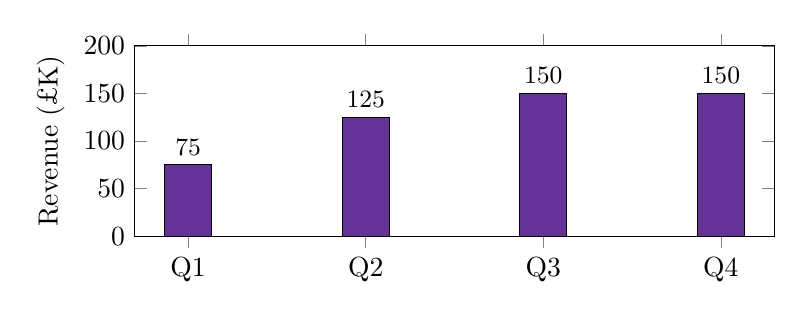
\begin{tikzpicture}
    \begin{axis}[
        width=0.8\textwidth,
        height=4cm,
        ybar,
        ylabel={Revenue (£K)},
        symbolic x coords={Q1,Q2,Q3,Q4},
        xtick=data,
        ymin=0,
        ymax=200,
        bar width=0.6cm,
        nodes near coords,
        every node near coord/.append style={font=\small}
    ]
    \addplot[fill=dreamlabprimary] coordinates {(Q1,75) (Q2,125) (Q3,150) (Q4,150)};
    \end{axis}
\end{tikzpicture}
\end{center}
\end{frame}

% Business Model
\begin{frame}{Business Model}
\begin{columns}
\column{0.6\textwidth}
\textbf{Revenue Streams:}
\begin{enumerate}
    \item \textbf{Project-Based} (40\%)
        \begin{itemize}
            \item £15K-£75K engagements
            \item 2-6 month delivery
        \end{itemize}
    \item \textbf{Retainers} (40\%)
        \begin{itemize}
            \item £3K-£8K monthly
            \item Ongoing optimisation
        \end{itemize}
    \item \textbf{Performance} (20\%)
        \begin{itemize}
            \item 10-20\% success fees
            \item Aligned incentives
        \end{itemize}
\end{enumerate}

\column{0.4\textwidth}
\textbf{Unit Economics:}
\begin{itemize}
    \item Gross Margin: \textbf{65\%}
    \item CAC: \textbf{£2,500}
    \item LTV: \textbf{£35,000}
    \item Payback: \textbf{3 months}
\end{itemize}
\end{columns}
\end{frame}

% Market Size
\begin{frame}{Market Opportunity}
\begin{center}
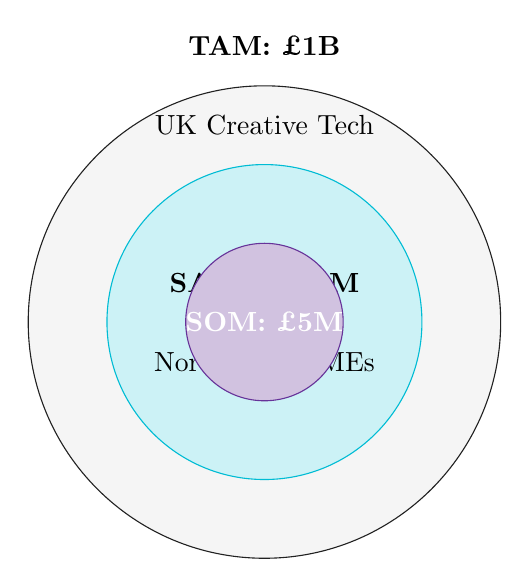
\begin{tikzpicture}
    % TAM
    \draw[fill=dreamlablight, draw=dreamlabdark] (0,0) circle (3cm);
    \node at (0,3.5) {\textbf{TAM: £1B}};
    \node at (0,2.5) {UK Creative Tech};
    
    % SAM
    \draw[fill=dreamlabaccent!20, draw=dreamlabaccent] (0,0) circle (2cm);
    \node at (0,0.5) {\textbf{SAM: £100M}};
    \node at (0,-0.5) {North-West SMEs};
    
    % SOM
    \draw[fill=dreamlabprimary!30, draw=dreamlabprimary] (0,0) circle (1cm);
    \node[white] at (0,0) {\textbf{SOM: £5M}};
\end{tikzpicture}
\end{center}

\textbf{5-Year Target:} 5\% of SAM = £5M ARR
\end{frame}

% Team
\begin{frame}{World-Class Team}
\begin{columns}
\column{0.5\textwidth}
\textbf{Leadership:}
\begin{itemize}
    \item \textbf{CEO}: 15+ years agency leadership
    \item \textbf{CTO}: Ex-Google, AI/ML expert
    \item \textbf{Creative Director}: BAFTA winner
    \item \textbf{CMO}: Built 3 successful agencies
\end{itemize}

\column{0.5\textwidth}
\textbf{Team Composition:}
\begin{itemize}
    \item 30 specialists across 10 disciplines
    \item 70\% senior-level (5+ years)
    \item Academic advisors from top universities
    \item Industry mentors from Fortune 500
\end{itemize}
\end{columns}

\vspace{0.5cm}
\begin{center}
\colorbox{dreamlabprimary!20}{\textbf{Combined 200+ years of experience delivering £50M+ in projects}}
\end{center}
\end{frame}

% Competitive Advantage
\begin{frame}{Sustainable Competitive Advantage}
\begin{enumerate}
    \item \textbf{Mesh Fluency}
        \begin{itemize}
            \item Only agency with true integration across AI + Immersive + Creative
            \item No handoffs, no silos, no delays
        \end{itemize}
    
    \item \textbf{Government Endorsement}
        \begin{itemize}
            \item GMCA innovation partner status
            \item University R\&D collaborations
            \item Access to grants and funding
        \end{itemize}
    
    \item \textbf{SME-First Pricing}
        \begin{itemize}
            \item Modular, scalable solutions
            \item 50\% lower than enterprise consultancies
            \item Performance-based options
        \end{itemize}
    
    \item \textbf{Regional Dominance}
        \begin{itemize}
            \item Deep North-West connections
            \item Local talent pipeline
            \item Lower operating costs than London
        \end{itemize}
\end{enumerate}
\end{frame}

% Go-to-Market
\begin{frame}{Go-to-Market Strategy}
\begin{columns}
\column{0.5\textwidth}
\textbf{Phase 1: Foundation (Q1)}
\begin{itemize}
    \item 3 pilot clients
    \item Core team assembly
    \item Brand launch prep
\end{itemize}

\textbf{Phase 2: Launch (Q2)}
\begin{itemize}
    \item Digital City Festival
    \item PR campaign
    \item 25 qualified leads
\end{itemize}

\column{0.5\textwidth}
\textbf{Phase 3: Scale (Q3-Q4)}
\begin{itemize}
    \item 15-20 active clients
    \item £500K revenue run rate
    \item Team expansion to 40
\end{itemize}

\textbf{Phase 4: Expand (Year 2)}
\begin{itemize}
    \item National presence
    \item £2M ARR
    \item Series A ready
\end{itemize}
\end{columns}
\end{frame}

% Financial Projections
\begin{frame}{Financial Projections}
\begin{center}
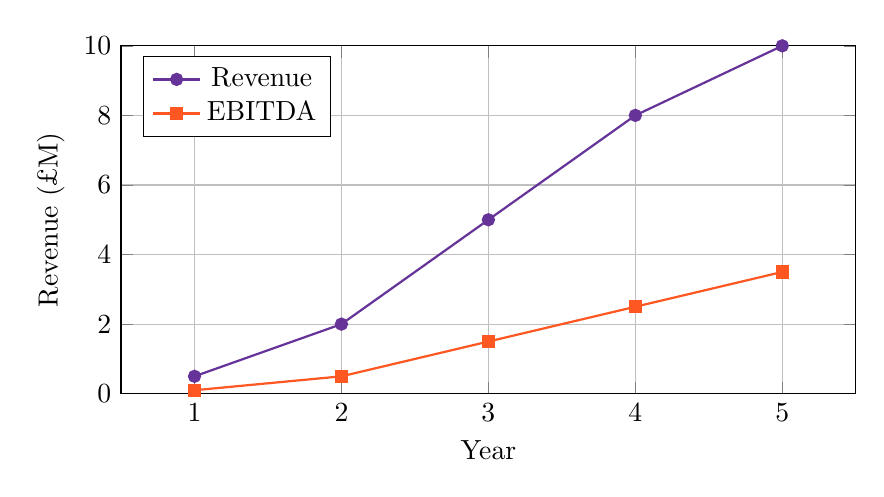
\begin{tikzpicture}
    \begin{axis}[
        width=0.9\textwidth,
        height=6cm,
        xlabel={Year},
        ylabel={Revenue (£M)},
        xmin=0.5, xmax=5.5,
        ymin=0, ymax=10,
        xtick={1,2,3,4,5},
        grid=major,
        legend pos=north west
    ]
    \addplot[color=dreamlabprimary, thick, mark=*] coordinates {
        (1,0.5) (2,2) (3,5) (4,8) (5,10)
    };
    \addlegendentry{Revenue}
    
    \addplot[color=dreamlabsecondary, thick, mark=square*] coordinates {
        (1,0.1) (2,0.5) (3,1.5) (4,2.5) (5,3.5)
    };
    \addlegendentry{EBITDA}
    \end{axis}
\end{tikzpicture}
\end{center}

\textbf{Key Metrics:}
\begin{itemize}
    \item Break-even: Month 6
    \item Gross Margin: 65\%+ maintained
    \item EBITDA Margin: 35\% by Year 3
\end{itemize}
\end{frame}

% Use of Funds
\begin{frame}{Use of Funds: £1.5M Seed Round}
\begin{columns}
\column{0.6\textwidth}
\begin{itemize}
    \item \textbf{Talent Acquisition (40\%)}
        \begin{itemize}
            \item 10 senior hires
            \item Key leadership roles
        \end{itemize}
    \item \textbf{Technology \& R\&D (25\%)}
        \begin{itemize}
            \item AI infrastructure
            \item Innovation lab setup
        \end{itemize}
    \item \textbf{Sales \& Marketing (20\%)}
        \begin{itemize}
            \item National expansion
            \item Brand building
        \end{itemize}
    \item \textbf{Operations (15\%)}
        \begin{itemize}
            \item Systems and processes
            \item Working capital
        \end{itemize}
\end{itemize}

\column{0.4\textwidth}
\begin{tikzpicture}
    \pie[text=legend]{
        40/Talent,
        25/Technology,
        20/Marketing,
        15/Operations
    }
\end{tikzpicture}
\end{columns}
\end{frame}

% Investment Terms
\begin{frame}{Investment Opportunity}
\begin{center}
\begin{tcolorbox}[colback=dreamlablight, colframe=dreamlabprimary, width=0.8\textwidth]
\textbf{\Large Seeking: £1.5M Seed Round}

\vspace{0.5cm}
\begin{itemize}
    \item Pre-money valuation: £3.5M
    \item Use of funds: Scale to £2M ARR
    \item Timeline: Close Q2 2025
    \item Lead investor: In discussions
\end{itemize}
\end{tcolorbox}
\end{center}

\vspace{0.5cm}
\textbf{Why Now?}
\begin{itemize}
    \item Market timing perfect (AI adoption curve)
    \item Proven model with early traction
    \item Team assembled and ready to scale
    \item Clear path to Series A (£5M ARR)
\end{itemize}
\end{frame}

% Exit Strategy
\begin{frame}{Exit Strategy}
\textbf{Potential Acquirers:}
\begin{columns}
\column{0.5\textwidth}
\begin{itemize}
    \item \textbf{Global Consultancies}
        \begin{itemize}
            \item Accenture Interactive
            \item Deloitte Digital
            \item PwC
        \end{itemize}
    \item \textbf{Agency Networks}
        \begin{itemize}
            \item WPP
            \item Publicis
            \item Omnicom
        \end{itemize}
\end{itemize}

\column{0.5\textwidth}
\begin{itemize}
    \item \textbf{Tech Platforms}
        \begin{itemize}
            \item Adobe
            \item Salesforce
            \item Microsoft
        \end{itemize}
    \item \textbf{Regional Leaders}
        \begin{itemize}
            \item The Hut Group
            \item Boohoo Group
            \item AO.com
        \end{itemize}
\end{itemize}
\end{columns}

\vspace{0.5cm}
\begin{center}
\colorbox{dreamlabsecondary!20}{\textbf{Target Exit: 5-7 years at 10x revenue multiple}}
\end{center}
\end{frame}

% Why DreamLab Will Win
\begin{frame}{Why DreamLab Will Win}
\begin{enumerate}
    \item \textbf{Perfect Timing}
        \begin{itemize}
            \item AI adoption hitting mainstream
            \item SMEs desperate for accessible innovation
        \end{itemize}
    
    \item \textbf{Unique Position}
        \begin{itemize}
            \item Only integrated AI + Immersive + Creative agency
            \item Government-endorsed credibility
        \end{itemize}
    
    \item \textbf{Proven Team}
        \begin{itemize}
            \item Built and sold agencies before
            \item Deep technical and creative expertise
        \end{itemize}
    
    \item \textbf{Clear Path to Scale}
        \begin{itemize}
            \item Repeatable sales process
            \item High-margin business model
            \item Multiple expansion opportunities
        \end{itemize}
\end{enumerate}
\end{frame}

% Call to Action
\begin{frame}{Join Us in Building the Future}
\begin{center}
\Large
\textbf{We're not just building an agency.}\\
\vspace{0.5cm}
\textbf{We're creating the blueprint for how businesses innovate.}
\end{center}

\vspace{1cm}

\begin{columns}
\column{0.5\textwidth}
\begin{center}
\faEnvelope\ invest@dreamlab.agency\\
\faPhone\ +44 161 XXX XXXX\\
\faGlobe\ dreamlab.agency
\end{center}

\column{0.5\textwidth}
\begin{center}
\faLinkedin\ /company/dreamlab\\
\faTwitter\ @dreamlabagency\\
\faMapMarker\ MediaCityUK, Salford
\end{center}
\end{columns}
\end{frame}

% Appendix
\begin{frame}{Appendix: Key Metrics Dashboard}
\small
\begin{table}
\centering
\begin{tabular}{l|r|r|r|r|r}
\toprule
\textbf{Metric} & \textbf{Y1} & \textbf{Y2} & \textbf{Y3} & \textbf{Y4} & \textbf{Y5} \\
\midrule
Revenue (£M) & 0.5 & 2.0 & 5.0 & 8.0 & 10.0 \\
Clients & 20 & 50 & 100 & 150 & 200 \\
Team Size & 30 & 50 & 80 & 120 & 150 \\
Gross Margin & 65\% & 65\% & 67\% & 68\% & 70\% \\
EBITDA Margin & 20\% & 25\% & 30\% & 32\% & 35\% \\
ARR (£M) & 0.3 & 1.2 & 3.0 & 5.0 & 7.0 \\
\bottomrule
\end{tabular}
\end{table}
\end{frame}

\end{document}